\def \secname {Polynomial Interpolation}

\section[\secname]{\hyperlink{toc}{\secname}}

\subsection{Lagrange Interpolation}

\begin{itemize}
    \item Notation: $(x_j, y_j) \equiv (x_j, f(x_j)) \equiv (x_j, f_j)$
    \item Goal: Given n Data points $(x_j, f_j) \qquad j=1,2,...,n$ find (construct) unique polynomial of (maximum) degree $n-1$ passing through all data points. (Degree is the largest power of independent variable).

    \[p(x) = \sum_{i=0}^{n-1} c_i x^i \qquad \text{where c is coefficients}\]

    This is a polynomial of (maximum) degree $n-1$
    \item Once $p(x)$ is determined can use to get approximate (interpolated) values of $(f(x))$ for $x_1 \le x \le x_n$

    \item Many representations of interpolating polynomial. Lagrange approach is to take:

    \[p(x) = \sum_{j=1}^{n} f_j l_j(x) \qquad \text{where the l term is of degree n-1}\]

    Where $l_j(x)$ are characteristic polynomial satisfying

    \[l_j(x_i) = \delta_{ji}\]

    Recall the $\delta_{ji} \equiv $ Kroenicker delta where it equals 1 if $i=j$ else it equals 0

    \item Then
 \[p(x_i) = \sum_{j=1}^{n} \frac{f_jl_i(x)}{\delta_{ji}} = \sum_{j=1}^n f_j \delta_{ji} = f_i\]

    \item Building characteristic polynomial
    \[ l_j(x) = \frac{(x-x_1)(x-x_2)...(x-x_{j-1})(x-x_{j+1})...(x-x_n)}{(x_j-x_1)(x_j-2)...(x_j-x_{j-1})(x_j-x_{j+1})...(x_j-x_n)}\] 
    \item Consider $l_j(x_i)=\delta_{ji}$

    \[i=j \rightarrow \text{numerator}=\text{denominator} \qquad l_j(x_j) = 1\]

    \[i \neq j \rightarrow \text{exactly one term in numerator vanishes, so } l_i(x_i) = 0 \]


    \begin{thmbox}{Final Formula: Lagrange Interpolating Polynomial}
        \begin{equation}
            p(x) = \sum_{j=1}^n f_j l_j(x)
        \end{equation}

        \begin{equation}
            l_j(x) = \prod_{i=1, \space i \neq j}^n \frac{(x-x_i)}{(x_j-x_i)} \qquad \text{$n^2$ number of calculations}
        \end{equation}
    \end{thmbox}
    
\end{itemize}
\subsection{Barycentric Interpolation}

Related to problem of determining centre of mass for a group of particles with given positions and weights.

\begin{itemize}
    \item First, define $l(x)$
    \[ l(x) = (x-x_1)(x-x_2)...(x-x_j)...(x-x_n)\]
    Then note that numerator at $l_j$ in (2) is $l(x)/(x-x_j)$
    \item Next, define Barycentric weights by
    \[w_j = \frac{1}{\prod_{i=1, \space i \neq j}^n (x_j-z_i)}\]

    \item Then Characteristic Polynomial $l_j(x)$ is $l_j(x) = l(x) \frac{w_j}{x-x_j}$

    \item Get the first formula for:
    
    \begin{thmbox}{Barycentric Interpolation}
        \begin{equation}
            p(x) = f(x) \qquad \sum_{j=1}^n \frac{w_j}{x-x_j} f_j \qquad \text{n number of operations}
        \end{equation}
    \end{thmbox}



    \item Advantage 
    \begin{itemize}
        \item Original $O(n^2)$ calculations to eliminate at any point.
        \item Barycentric: $O(n^2)$ to compute weights, $O(n)$ to evaluate
    \end{itemize}
    
    \item Another version: let all $f_j = 1$ then from (1) AND (3)
    \[1 = \sum_{j=1}^n l_j (x) = l(x)\sum_{j=1}^n \frac{w_j}{x-x_j}\]

    \item Divide (3) by last result, cancel $l(x)$ Term

    \begin{thmbox}{Barycentric Interpolation Version 2}
        \begin{equation}
            p(x) = \sum_{j=1}^n \frac{w_j}{x-x_j} f_j / \sum_{j=1}^n \frac{w_j}{x-x_j}
        \end{equation}
    \end{thmbox}
\end{itemize}

\subsection{Numerical Example (EXAM HINT)}

!!!!!!!!!!!!!!!!!!!!!!!!!!!!!!!!!!!!!!!!!
\begin{itemize}
    \item Use (1), (2) to construct degree-2 Polynomial passing through (-1,6), (1,8), (3,34) for 
\end{itemize}

\[p(x) = \sum_{j=1}^n f_j l_j(x) \]

\[l_j(x) = \prod_{i=1, \space i \neq j}^n \frac{(x-x_i)}{(x_j-x_i)} \qquad \text{$n^2$ number of calculations}\]

\[ p(x) = 6 \frac{(x-1)(x-3)}{(-1-1)(-1-3)} + 8 \frac{(x+1)(x-3)}{(1+1)(1-3)} + 34 \frac{(x+1)(x-1)}{(3+1)(3-1)}\]

\[ p(x) = 6 \frac{(x-1)(x-3)}{8} + 8 \frac{(x+1)(x-3)}{-4} + 34 \frac{(x+1)(x-1)}{8}\]

\[ p(x) = 3\frac{(x-1)(x-3)}{4} + -2 (x+1)(x-3) + 17 \frac{(x+1)(x-1)}{4}\]


Let me check my answer by plotting the points and the result polynomial equation:


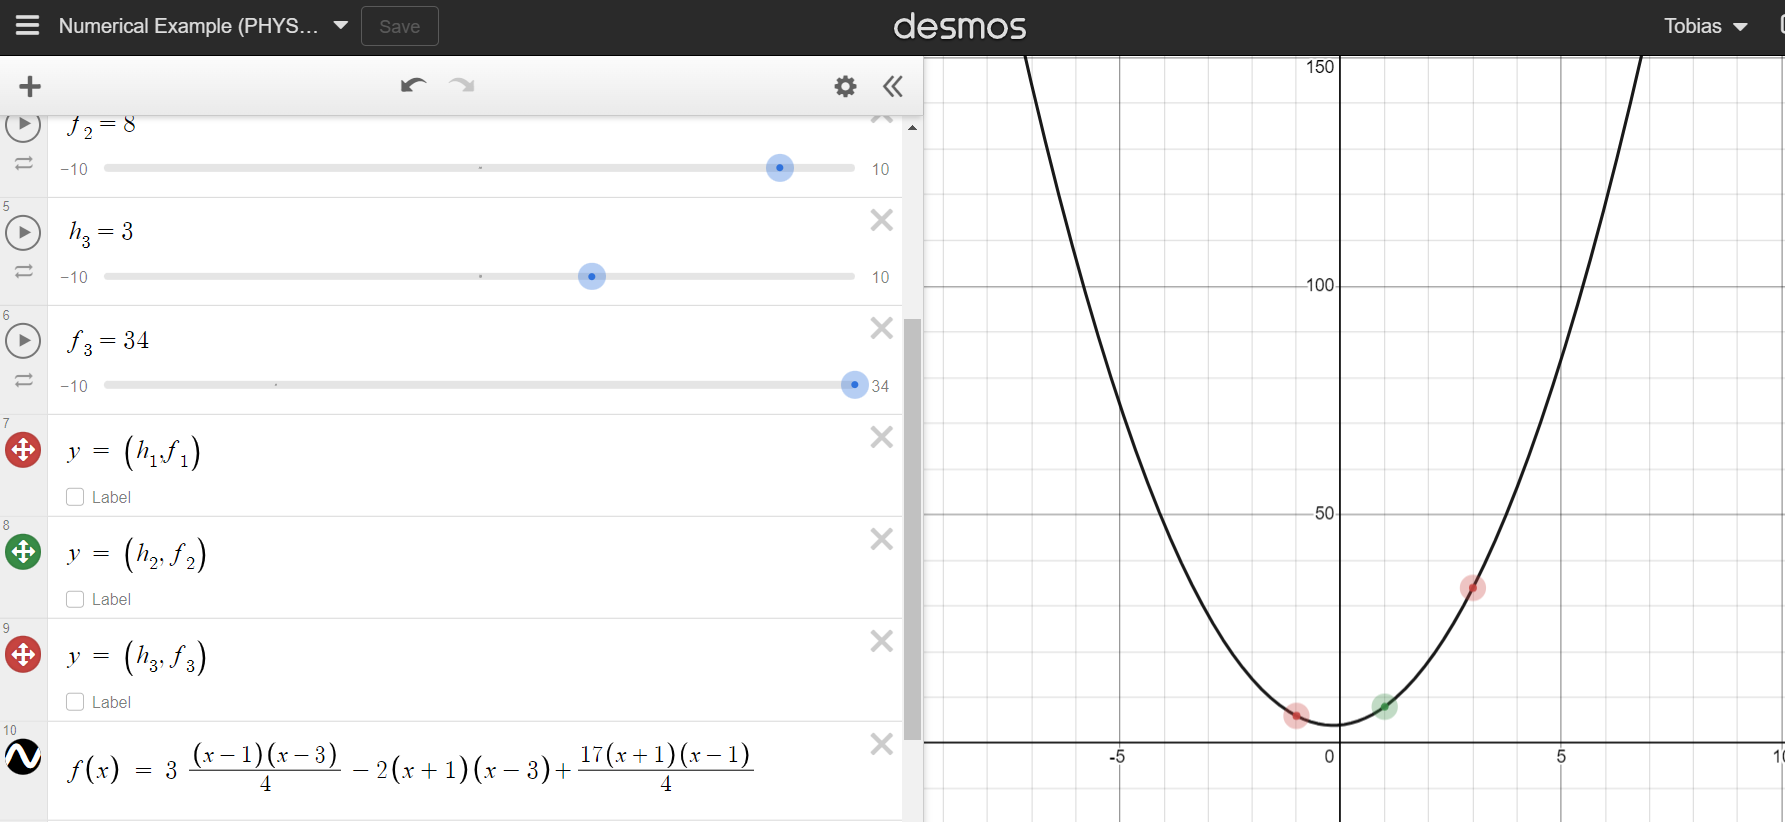
\includegraphics[width = \linewidth]{Images/NumericalExample_LagrangePolyInterp.png}

!!!!!!!!!!!!!!!!!!!!!!!!!!!!!!!!!!!!!!!!!

\subsection{Symbolic Example}
\begin{itemize}
    \item Consider 3 equi-spaced data points:
    \[(-h,f_{-1}), (0,f_0), (+h,f_1)\]

    \item Using (1), (2), Construct a lagrange interpolating polynomial and evaluate it's derivative at x=0

    \begin{equation*}
    \begin{aligned}
        p(x) &= \sum_{j=1}^3 f_j l_j(x)\\
        &= f_{-1}\frac{x(x-h)}{(-h)(-2h)} + f_0 \frac{(x+h)(x-h)}{(h)(-h)} + f_1 \frac{(x+h)(x)}{(2h)(h)}\\
        &= f_{-1} \frac{x^2-hx}{2h^2} - f_0 \frac{x^2-h^2}{h^2} + f_1 \frac{x^2+hx}{2h^2}
    \end{aligned}
    \end{equation*}

    \begin{equation*}
        \left. \frac{d(p(x)}{dx} \right\vert_{x=0} = \frac{f_1-f_{-1}}{2h} \rightarrow \text{Finite difference approximation for } f'(x)
    \end{equation*}
    
\end{itemize}
